\documentclass{beamer}

%% Juego de caracteres usado en el archivo fuente: UTF-8
\usepackage{ucs}
\usepackage[utf8x]{inputenc}
\uselanguage{spanish}
%Para la identación del español
\usepackage[spanish]{babel}
\usepackage{eurosym}

% There are many different themes available for Beamer. A comprehensive
% list with examples is given here:
% http://deic.uab.es/~iblanes/beamer_gallery/index_by_theme.html
% You can uncomment the themes below if you would like to use a different
% one:
%\usetheme{AnnArbor}
%\usetheme{Antibes}
%\usetheme{Bergen}
%\usetheme{Berkeley}
%\usetheme{Berlin}
%\usetheme{Boadilla}
%\usetheme{boxes}
%\usetheme{CambridgeUS}
%\usetheme{Copenhagen}
%\usetheme{Darmstadt}
%\usetheme{default}
%\usetheme{Frankfurt}
%\usetheme{Goettingen}
%\usetheme{Hannover}
%\usetheme{Ilmenau}
%\usetheme{JuanLesPins}
%\usetheme{Luebeck}
\usetheme{Madrid}
%\usetheme{Malmoe}
%\usetheme{Marburg}
%\usetheme{Montpellier}
%\usetheme{PaloAlto}
%\usetheme{Pittsburgh}
%\usetheme{Rochester}
%\usetheme{Singapore}
%\usetheme{Szeged}
%\usetheme{Warsaw}

%Para la identación del español
\usepackage[spanish]{babel}

\title{Proyecto robótico}

% A subtitle is optional and this may be deleted
%\subtitle{Optional Subtitle}

\author{Juan Pedro Rodríguez Gracia \\ Jesús Rodríguez Heras \\ Gabriel Fernando Sánchez Reina}
% - Give the names in the same order as the appear in the paper.
% - Use the \inst{?} command only if the authors have different
%   affiliation.

%\institute[Escuela Superior de Ingeniería] % (optional, but mostly needed)
%{
%  \inst{1}%
%  Department of Computer Science\\
%  University of Somewhere
%  \and
%  \inst{2}%
%  Department of Theoretical Philosophy\\
%  University of Elsewhere}
% - Use the \inst command only if there are several affiliations.
% - Keep it simple, no one is interested in your street address.

\date{13 de febrero de 2018}
% - Either use conference name or its abbreviation.
% - Not really informative to the audience, more for people (including
%   yourself) who are reading the slides online

%\subject{Theoretical Computer Science}
% This is only inserted into the PDF information catalog. Can be left
% out. 

% If you have a file called "university-logo-filename.xxx", where xxx
% is a graphic format that can be processed by latex or pdflatex,
% resp., then you can add a logo as follows:

% pgfdeclareimage[height=0.5cm]{university-logo}{university-logo-filename}
% \logo{\pgfuseimage{university-logo}}

% Delete this, if you do not want the table of contents to pop up at
% the beginning of each subsection:
%\AtBeginSubsection[]
%{
%  \begin{frame}<beamer>{Índice}
%    \tableofcontents[currentsection,currentsubsection]
%  \end{frame}
%}

% Let's get started
\begin{document}

\begin{frame}
  \titlepage
  
  
\end{frame}

\begin{frame}{Índice}
  \tableofcontents
  % You might wish to add the option [pausesections]
\end{frame}

% Section and subsections will appear in the presentation overview
% and table of contents.
\section{Objetivo}
\begin{frame}{Objetivo}
	\begin{block}{¿Cuál es el objetivo?}
		El objetivo de este proyecto es la obtención de un robot móvil capaz de salir de un laberinto por sí mismo y estar dotado de la inteligencia suficiente como para volver a la casilla inicial por el recorrido más corto.
	\end{block}
\end{frame}

\section{Hardware empleado}
\begin{frame}{Hardware empleado}
	Para conseguir el objetivo del proyecto hemos utilizado el siguiente hardware:
	\begin{itemize}
		\item Arduino Leonardo.
		\item Sensor de ultrasonidos.
		\item Sensor de infrarrojos.
		\item CNY's.
		\item Motores.
		\item Antena bluetooth.
		\item Batería.
	\end{itemize}
\end{frame}

\section{Montaje}
\begin{frame}{Montaje}
	En cuanto al montaje optamos por un diseño funcional el cual hemos impreso en una impresora 3D del laboratorio obteniendo este resultado:\\
	\begin{center}
		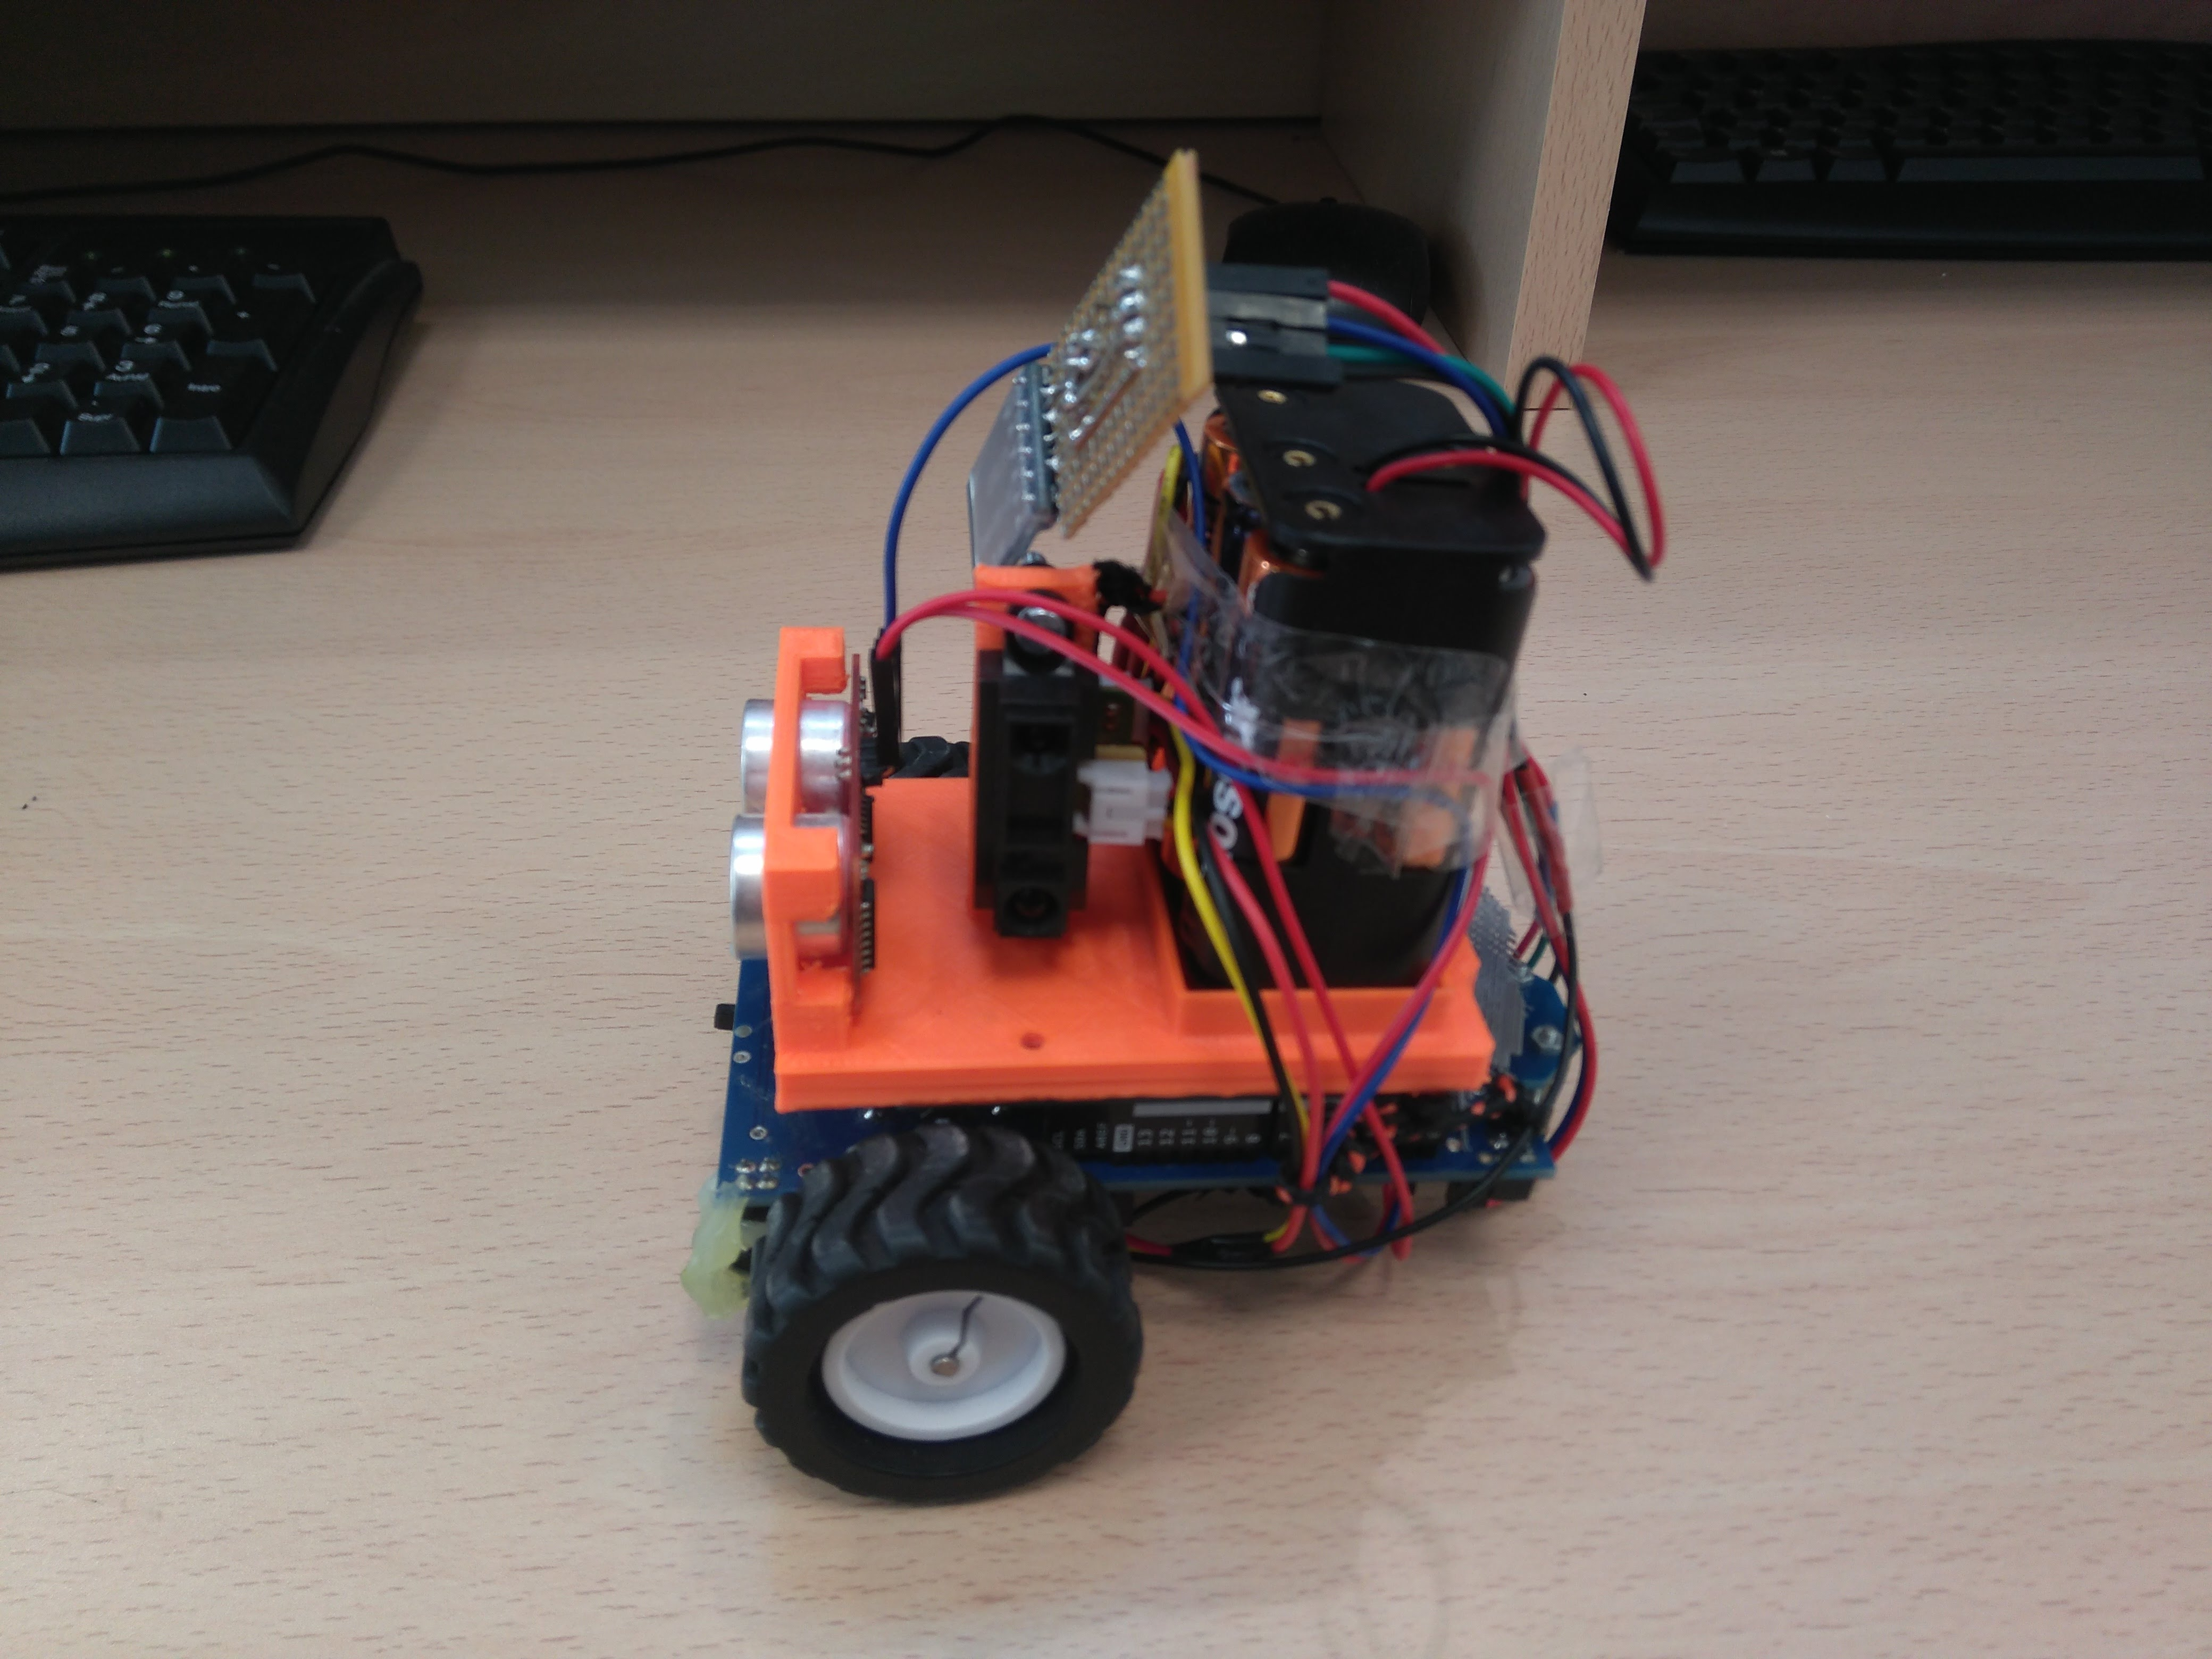
\includegraphics[scale=0.05]{F1.jpg}
	\end{center}	
\end{frame}

\section{Requisitos}
\begin{frame}{Requisitos}
\begin{itemize}
	\item El robot es capaz de moverse en todas direcciones reconociendo paredes y líneas.
	\item Es capaz de realizar giros de 90º y 180º.
	\item Es capaz de volver al inicio cuando reconoce que ha llegado a la meta.
	\item Mediante la conexión bluetooth es capaz de enviar el camino que va recorriendo al ordenador portátil el cual lo representará en una interfaz gráfica.
\end{itemize}
\end{frame}



\section{Implementación}
\begin{frame}{Implementación}
	Para la implementación software hemos usado el lenguaje C++ para el funcionamiento del robot y Python para la comunicación bluetooth con el portátil.
\end{frame}

\section{Funcionamiento}
\begin{frame}{Funcionamiento}
\begin{block}{¿Cómo funciona?}
	Para la resolución del laberinto hemos usado el algoritmo de la mano derecha apoyándonos en una pila para calcular el camino de vuelta.
\end{block}	
\end{frame}

\section{Presupuesto}
\begin{frame}{Presupuesto}
	\begin{table}[htbp]
		\begin{center}
			\begin{tabular}{|c|c|c|}
				\hline 
				\textbf{Componente} & \textbf{Unidades} & \textbf{Precio total (\euro)}  \\
				\hline
				Arduino Leonardo & 1 & 18 \\\hline
				Placa Shield PCB & 1 & 25 \\\hline
				Sensor CNY70 & 3 & 5.10 \\\hline
				Sensor HC-SR04 & 1 & 1.49 \\\hline
				Cables & Varios & 1.20 \\\hline
				Módulo bluetooth GW040 & 1 & 7.73 \\\hline
				Motores Micro Metal & 2 & 27.80 \\\hline
				Sensor SHARP & 2 & 21.58 \\\hline
				Plástico & 20g & 1.46 \\\hline
				Pilas & 6 & 7.33 \\\hline
				Horas & 180 & 20€/hora \\\hline
			\end{tabular}
%			\caption{Presupuesto del proyecto.}
%			\label{tabla:Presupuesto del proyecto}
		\end{center}
	\end{table}	
	El presupuesto total ascendería a 3716,69\euro.
\end{frame}



\end{document}


